

%interpretation of results
\section{Interpretation of Results}
%interpreting EKF results
\subsection{EKF likelihood}
 In section~\ref{sec: EKF test} I found that the likelihood obtained using the Extended Kalman filter performs slightly worse than the Euler-Maruyama method for the parameters $\beta_1$ and $\beta_2$. A reason for this might be that the method was tested in a scenario where the Brownian motion is much larger than the drift in the Langevin process, which is what one might expect in an animal setting. This makes the predict steps of the extended Kalman filter undershoot the steps of the Langevin process. In turn, this leads to an error, which is compounded every time the predict step is performed. If the position used in the predict step is wrong, the prediction of the covariance using the curvature of the covariates also becomes wrong. To see how the extended Kalman filter works in practice, I used the covariates from earlier and plotted the predict steps of the Langevin process together with steps of the extended Kalman filter, and the 90\% confidence level using the predicted covariance. The results are shown in figure~\ref{fig:EKF high diffusion}. 


\begin{figure}[H]
    \centering
    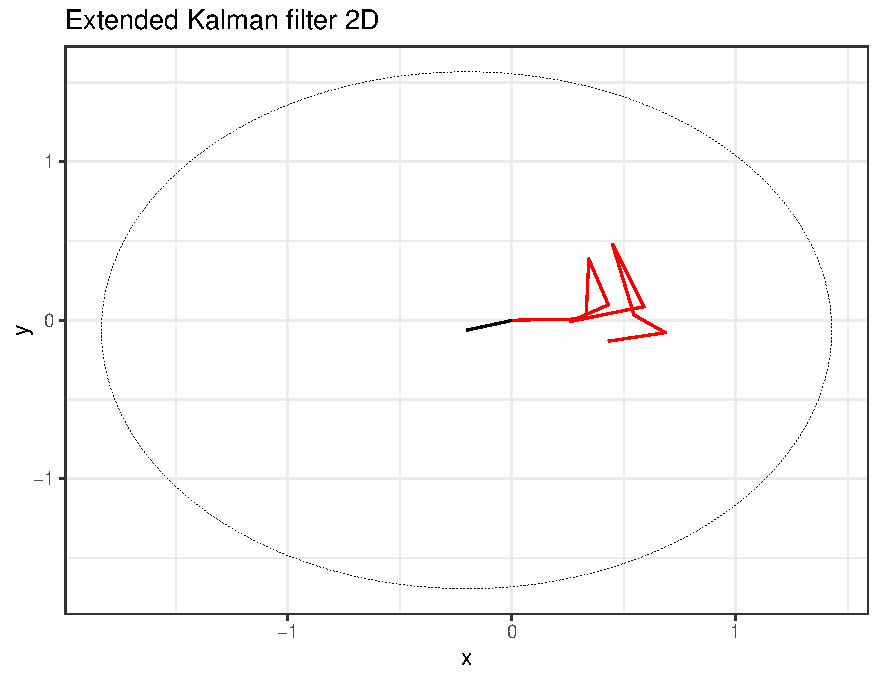
\includegraphics[width=\linewidth]{Images/discussion/EKF high diffusion path.pdf}
    \caption[Extended Kalman filter path]{Plot of extended Kalman filter state estimates. The black line shows the predicted state estimates over a time grid from 0 to 0.1, with increments 0.01. The dotted elipse shows the 90\% confidence level set of the final predicted state, and the red line show the Langevin process that is beeing estimated. The parameters used are the same for the Langevin process and the EKF}
    \label{fig:EKF high diffusion}
\end{figure}

Figure~\ref{fig:EKF high diffusion} shows that there is little correspondence between the path of the predictions made by the extended Kalman filter and the Langevin process. In this case, the paths have ended up going in almost opposite directions. This happens because the Langevin process pictured is dominated by randomness, which also means that the Langevin path is much longer than the path from the extended Kalman filter. Since the intermediate values of extended Kalman filter do not approximate the intermediate values of the Langevin process wee, doing multiple steps of the extended Kalman filter might not make an improvement to the estimate.
The extended Kalman filter might work better. Using intermediate predict steps in the extended Kalman filter might work better in scenarios where the diffusion is smaller and the drift larger, since the predictions would deviate less from the true values of the Langevin process.

\


%interpreting results from scenario 1
\subsection{Scenario 1}
\label{subsec: Scenario 1 interpretation}
In Scenario 1 in Section~\ref{sec: BB test} we saw that the method using the Brownian bridge importance sampling likelihood eliminated the bias observed in the estimates using the Euler-Maruyama method in figure~\ref{fig:EM_thin_boxplot}. This is not surprising because the importance sampling estimate should converge to the correct value of the likelihood and because the proposal being used is similar to the Langevin process. The test also showed that there were two estimates that overestimated the value of the parameter $\gamma^2$ by a large margin. This might be due to the method that was used to find the maximum likelihood estimate. The maximum likelihood was found by using the "L-BFGS-B" method implemented in the R-package "optim", and the likelihood function simulated new Brownian bridges each time it was evaluated. This meant that there was stochasticity in the likelihood, which could mean that optimization algorithm found a value of the likelihood that had a high value because of randomness. The estimates that were found were still an improvement on the estimates using the Euler-Maruyama method, but they could perhaps be improved further by simulating standard Gaussian variables $\textbf{Z}$ beforehand, then transforming them by using $\gamma \textbf{Z} +\mu$ to give Brownian bridges scaled with the right speed parameter. The likelihood estimates obtained by doing this would be deterministic, which might reduce the variance of the estimates, and hinder outliers.

\

Another observation from scenario 1 is that the variance of the $\bm \beta$-parameters is reduced as the time difference of the observations is increased, when the number of observations is held constant. This was observed both when the Brownian bridges were an were not pre-computed. The same explanation as was used to explain the same phenomenon for the Euler-Maruyama estimates, can be used in this case: that when more of the covariate range is explored, the variance of the coefficient estimates is reduced. Since estimates are unbiased at all values of $dt$, this suggests that If we are given the choice between a higher frequency of observations of an animals movement or a lower frequency, we should prefer the lower frequency, given that they have the same cost to acquire.

\

In scenario 1 in section~\ref{sec: BB test} we saw that the estimator using the precomputed Brownian bridge importance sampling likelihood is an improvement on the Euler-Maruyama estimates, for all the parameters. at a thinning of 10 there is little to no bias in the estimates, whereas using the Euler-Maruyama method there is an observable bias at this value of $\Delta_t$. For the speed parameter $\gamma^2$, we saw that there is a bias which is observed for thinning of 50 and 100. in both of these cases all the estimations done significantly underestimated the value of the parameter. One reason for this must be that the Brownian bridges become a much worse proposal density when the speed parameter used for generating the Brownian bridges deviates from the parameter which is being used to compute the likelihood. 
When $\Delta_t=0.1$ there is bias in the Euler-Maruyama method whose $\gamma^2$-estimates are used to simulate the Brownian bridges, however there is no bias in seen in figure~\ref{fig:varying dt boxplot precomputed BB} for this value of $\Delta_t$. This suggests that even if the value used to generate the bridges is slightly off, the likelihood can still be accurately approximated using this proposal, but for larger discrepancies, the method breaks down. 


\

A striking feature of the estimations done in using pre-computed Brownian bridges, is that even though there is a large bias in the speed parameter $\gamma^2$, there appears to be little or no bias in the estimates of $\bm \beta$. This is particularly interesting, since the drift term in the Langevin process is scaled by $\gamma^2$. This might suggest that the variance used in making the Brownian bridges is not important when it comes to estimating $\bm \beta$, but is more important when it comes to estimating $\gamma^2$. The fact that there is still bias 




%interpretation of scenario 2
\subsection{Scenario 2}
\label{subsec: scenario 2 interpretation}

In the simulations done in scenario 2 we saw that both when using and not using pre-computed Brownian bridges, there is a bias in the estimates of $\beta_1$ and $\beta_2$ when the number of nodes in the bridges becomes small. Interestingly, this is the opposite of the bias seen in the Euler-Maruyama estimates. As the number of nodes in the bridges decreases, one would think that the importance sampling estimates should approach that of the Euler-Maruyama estimates, since we would get the same error with the discretization. It is dificult to say exactly why this is not observed. For the $\gamma^2$ estimate when not using pre-computed bridges, we do observe what we would expect from the Euler-Maruyama method: that there is a bias toward zero.




%interpretation of scenario 3
\subsection{Scenario 3}
\label{subsec: scenario 3 interpretation}


When not using pre-computed bridges, we saw in scenario 3  that for small M, there was a bias in the estimates. One reason for this might be that the number of bridge nodes $N$ used, was less than the number of steps used to simulate the data. However as $M$ increased this bias disappeared. This can be explained by the fact that, even if we are using a non-optimal proposal density, the importance sampling estimate should still converge to the correct likelihood as $M$ increases. It also suggests that even if the number of bridge nodes $N$ is not enough to simulate the Langevin process, if we have enough of these bridges, we can still get unbiased estimates. Another observation from scenario 3 is that the variance of the estimates decreases as $M$ increases. This makes sense since when we are using more bridges, we are averaging over more paths to find the likelihood.

\

%precomputed
When using pre-computed bridges, the same pattern was seen. For a small number of bridges, there were large biases for $\beta_1$, $\beta_2$, and $\gamma^2$. However, as $M$ increased, the biases seen in $\beta_1$ and $\beta_2$ were eliminated, and the bias seen in $\gamma^2$. For all values of $M$ tried, there was a bias in $\gamma^2$, but it is reasonable to think that if $M$ becomes large enough, the bias seen in $\gamma^2$ when using pre-computed Brownian bridges will disappear once $M$ becomes large enough. This might mean that pre-computing the bridges might still be the better method if it can make up for the fact that more bridges are simulated by the fact that it is faster.


\subsection{Computation Time}

In subsection~\ref{subsec: computation time} we found that the for the given scenario, the average computation time using pre-computed Brownian bridges was 9.901651 minutes and when not using pre-computed bridges it was 18.8885 minutes. This means that there was some efficiency to be gained from pre-computing the Brownian bridges. However, since using pre-computed Brownian bridges gives the wrong estimates, this method should not be preferred over the alternative. As was discussed about scenario 3, the method using pre-computed Brownian bridges might give unbiased estimates is the number of bridges used is sufficiently high, and the efficiency gain of pre-computing the bridges might make up for the fact that more bridges have to be computed.

\

The standard deviation of the computation time when using pre-computed Brownian bridges was 0.504986 minutes and when not using pre-computed bridges it was  4.4879 minutes. One explanation for the larger deviation in computation time when not pre-computing the bridges might be that the likelihood in this case is stochastic. This might make the optimization algorithm find a point that by chance has a high value, which would make it stop early. Beacause of this, as mentioned eralier, simulating standard Brownian bridges, then scaling them when computing the likelihood, might be better for likelihood maximization.





\section{Limitations and Future Directions}
The method using Brownian bridge importance sampling showed promising results when it comes to eliminating the bias seen in the Euler-Maruyama method. A problem with using this method however, is that it cannot handle observation error. typically track data is collected with some observation error, for example from getting positions by GPS. If this error is not accounted for, the estimates would no longer be accurate. \parencite{michelot_langevin_2019} circumvents this problem by using the Kalman Filter to find predicted positions that are then used to estimate the parameters. Another possibility is that, when the distance between observations becomes large, the effect of the observation error on parameter estimates becomes less significant. This is something that would need to be studied further though. Alternatively, appendix~\ref{Appendix: Langevin with obs error} contains a derivation of a likelihood estimator for the Langevin process with normally distributed observation error. I have not made this estimator work in practice, which is why it is not in the main section of this thesis.

\

To study the estimates using the Brownian bridge importance sampling likelihood the Brownian bridges were simulated each time evaluating the likelihood. As mentioned in subsection~\ref{subsec: brownian bridge interpretation}. This was done because during testing there seemed to be a considerable speedup using this method. A study which was not performed in this thesis was to see how the estimates found by computing Brownian bridges each time evaluating the likelihood compared to estimates found by simulating Brownian bridge variables $Z$ beforehand, then transforming it using $\gamma X +\mu$. Where $\mu$ is the mean of the bridge between to observations, and $\gamma^2$ is the speed parameter that we scale the bridge by. Scaling the bridges instead of simulating them would give a deterministic likelihood, which might be better for optimization.

\

In addition to this the gradient used to optimize the Brownian bridge importance sampling likelihood was approximated by not taking the derivative by treating the bridges if they were not dependent on $\gamma^2$. Alternatively the gradient can be approximate numerically, which would require the Brownian bridges to scaled instead of re-simulated. In this thesis There were done no test to see if a numerical approximation of the gradient would give a different result to the likelihood maximization.

\

In this thesis i have not explored how to choose the number of bridge nodes $N$ or the number of bridges $M$ that should be used in the Brownian bridge importance sampling likelihood to eliminate the bias and reduce the variance of the estimator. If the number of bridge nodes $N$ is low, the estimates become biased,  however this can be compensated for by using more bridges. To see that the values of $N$ and $M$ are large enough, multiple values should be tried when fitting the model. if $M$ and $N$ are large enough, there should be small changes in the estimate when increasing their values. 

\

Often animal movement can be time dependent. For example an animals utilization distribution could change seasonally. The Langevin model does not support time-varying covariates, so this is something that would be unfeasible to model using it. It is however possible to use a time varying speed parameter $\gamma^2$. Changes in animal movement which occur on shorter time scales, and which do not affect the utilization distribution could therefore be modeled. The variance of the speed parameter is not reduced for lower frequency sampling. future research could therefor include what the effect of low frequency sampling is on the ability to model the speed.

\

Another topic that was not explored in tghis thesis is which proposal to use in importance sampling. In addtion to using Brownian bridges as a proposal, they also use what they call a "modified Brownian bridge" which has a variance that decreases as the bridge goes from the start to the endpoint. They show that this works better than Brownian bridges. There might also be other improvements that can be made, like using other forms of interpolation that linear interpolation for the mean of the bridges. 

\

using monte carlo integration of SSA might be better than metropolis hasting correction because ... There is information between the observations ... 
the langevin model is a very simple model for animal movement and may not be able to model direction persistance correctly
